\chapter{HybridCheck}
\label{chap:HC}

This chapter is based on the published scientific paper:

\vspace{5mm}

\textit{Ward, B. J., \& van Oosterhout, C. (2016). Hybridcheck: Software for the rapid detection, visualization and dating of recombinant regions in genome sequence data. Molecular Ecology Resources, 16(2), 534-539.}

\vspace{5mm}

The project and items of work were initially set out by my supervisor, but the work I present in this chapter is entirely my own work.
I drafted the pseudo-code for the project, improved the dating algorithm presented in the chapter from it's original inefficient design, wrote all the software code, documented the package, and conducted all simulations used to test the software package, and created a website, github repository, and a web-app which provides an interface for the package.


\newpage


\section{Introduction}

Recombination is one of the five evolutionary forces and is important for the formation of novel genotypes, haplotypes and alleles, thereby playing a key role in adaptive evolution \parencite{Grauer2000}. Recombination is also crucial for separating deleterious mutations from their genomic background, and in combination with purifying selection it helps to curtail the mutational load \parencite{Lynch1990a}. Recombination plays a fundamental role in the repair of damaged DNA, when homologous recombination replaces a damaged DNA strand with its intact counterpart. In all likelihood, it was this function of recombination that was important in early prokaryotic life and evolution \parencite{Cavalier-Smith2002}. With respect to adaptive evolution, however, the principal consequence of recombination is that it generates novel combinations of nucleotides, which in turns allows for selection to act a much finer scale, i.e. at the level of nucleotides rather than the entire genome. Given its fundamental importance in the biology, various mechanisms have evolved that facilitate recombination; with some depending on sexual reproduction whereas others also occur in asexually reproducing taxa. As evolutionary biologists/molecular ecologists studying gene and genome sequences, it is important to understand how the various mechanisms can result in recombination.

Homologous recombination is a process that occurs in both eukaryotes and prokaryotes, and it is an essential process through which single strand and double strand breaks, as well as base mismatches in DNA molecules are repaired. With homologous recombination, there is an equal exchange of homologous DNA sequences between the two chromatids \parencite{Lemey2009b}. In eukaryotes, this can occur through Double Strand Break Repair (DSBR) and Synthesis Dependent Strand Annealing (SDSA) \parencite{McMahill2007Synthesis-dependentMeiosis.,Sung2006MechanismFunctions}. In prokaryotes, the RecBCD pathway, and the RecF pathways are the primary mechanisms \parencite{Madigan2012,Smith2012}. Although these pathways differ mechanistically, they all result in the invasion of donor DNA into a recipient DNA molecule through the formation of Holliday junctions, branch migration, ligation, and the repair of the DNA strands \parencite{Alberts2002}.

The precise outcome of recombination and its effect on the donor and recipient DNA molecule depends on how the Holliday junctions are cut and resolved \parencite{Mimitou2009}.
Crossing-over or reciprocal homologous recombination occurs when there is an equal exchange of sequence variation between the two homologous chromosomes \parencite{Grauer2000}.
Gene conversion is a type of non-reciprocal homologous recombination in which there is an unequal exchange of one sequence (the donor) to another (the recipient), such that the donor sequence replaces the recipient DNA \parencite{Grauer2000}.
Whereas crossing-over does not affect nucleotide variation, gene conversion tends to reduce nucleotide variation by making the donor and recipient sequence identical to one another.
However, even though gene conversion tends to homogenise nucleotide variation, this process too can increase haplotype and genotype variation in the population, just like crossing-over \parencite{Spurgin2011}.
Both reciprocal and non-reciprocal recombination can occur between non-homologous sequences \parencite{Lemey2009b}.
In addition, recombination can occur when distinct species or biotypes hybridise, in which case it is referred to as genetic introgression \parencite{McMullan2015a}.
Genetic exchange between even more distantly related taxa can result in horizontal gene transfer \parencite{Eisen2000,Ochman2000}.
This too is considered a form of recombination, which occurs after gene flow between distinct taxa, and bacterial geneticists most commonly use the term 'horizontal gene transfer'.

Recombination can complicate evolutionary genetic, phylogenetic and phylogenomic analyses because neighbouring nucleotides within a single genome can differ markedly in their ancestry and coalescence.
In the absence of recombination, the ancestry of a multiple alignment of homologous sequences can be represented by a single gene phylogeny. 
However, after a single recombination event, the sequences could have a different phylogenetic history and thus different phylogenies either side of the breakpoint \parencite{Lemey2009c}.
Each recombinant region between two breakpoints could have a distinct ancestry and be represented by a different phylogeny.
With high recombination rates, the history of a set of sequences becomes increasingly complex as different portions of the genome are shuffled, resulting in overlapping regions with distinct coalescence \parencite{Jouet2015}.
If recombination occurs in a single panmictic population, however, there will be relatively little variation in the ancestry of recombinant regions because all sequences coalesce relatively recently.
On the other hand, recombination in structured populations (e.g. between distinct biotypes, strains or races) may result in the genetic introgression of diverged donor sequences, and this can lead to a mosaic-like genome structure \parencite{McMullan2015a}.
In such cases, it is inappropriate to force a single phylogenetic tree onto a mosaic-like sequence, and it has been shown that this can significantly bias estimates of coalescent times \parencite{Jouet2015}.
Not only phylogenetic analyses are hindered by recombination, but also population genetic statistics can become biased if recombination is not accounted for, for example resulting in an upwards biased estimate of theta (and hence the effective population size) \parencite{McVean2002,Watterson1975}, and the erroneous identification of positive selection \parencite{SHRINER2003}.

Given that recombination can potentially affect population genetic, evolutionary genetic and phylogenetic analyses, it is important to examine whether recombination has left a signature in the sequence data. There are probably three questions one might address when analysing recombination in genome sequence data:

\begin{enumerate}
	\item Is there evidence of recombination?
    \item Where are the breakpoints / regions of recombination located in the sequence?
    \item What is the rate of recombination scaled relative to the mutation rate or theta?
\end{enumerate}

To detect the evidence for recombination, graphical exploratory tools can be used such as Splitstree \parencite{Huson2006}, which visualises the impact of recombination on the phylogenetic relationship between alleles or sequences. However, to formally test the evidence of recombination, statistical tests need to be used, and many algorithms have been developed for this purpose \parencite{Lemey2009b,Lemey2009c}. The general rationale of these tests is that recombination can insert novel nucleotides into a sequence alignment, making it appear that these polymorphisms have arisen there by mutation. A single nucleotide polymorphic (SNP) that is shared between two sequences, but which is not shared with their common ancestor is called a homoplasy. Such homoplasies are explained either by recombination or convergent evolution \parencite{MaynardSmith1998}. Statistical methods for detecting recombination are based on detecting phylogenetic incompatibilities that result from homoplasies \parencite{Bruen2006,Posada2002}, or by finding clusters of identical substitutions in sequences \parencite{Posada2002}. Measures that are computed by such methods, such as for example the homoplasy test \parencite{MaynardSmith1998}, the informative sites test \parencite{Worobey2001a}, the refined incompatibility score \parencite{Bruen2006}, and the ABBA BABA test \parencite{SMartin2014,Green2010a} can be used to evaluate whether recombination has taken place. For example, ABBA BABA tests classify homoplasious SNPs as having one of two possible parsimonious ancestries, and they calculate the Patterson’s D statistic that is based on the ratio of both types of ancestries. In case there is a significant excess of one type of ancestry over the other, this is considered evidence of recombination.

Once it has been established that recombination is affecting a nucleotide sequence, one can employ methods to identify where in the genome recombination has taken place. Those methods generally implement a scanning sliding window, and they calculate for each window the distribution of nucleotide substitutions or the genetic distance, or they assess the phylogenetic relationships between sequences at the window \parencite{Lemey2009c,Posada2002}. The former two methods typically attempt to find inversions or sudden changes in substitution pattern or distance values across the windows, and they do not rely on a phylogeny. Phylogenetic methods, on the other hand, infer recombination by detecting changes in the topologies, i.e. the shape of the tree. If adjacent sections of DNA sequence are phylogenetically incongruent, this is evidence for a recombination event or breakpoint \parencite{Lemey2009b}. Methods that rely on sliding windows tend to be hampered by an increased false positive rate (Type I error rate) due to multiple testing \parencite{Lemey2009b}. Bayesian approaches \parencite{Paraskevis2005} have been developed to avoid such sequential testing problems, and in addition, they can identify breakpoint positions and the parental (donor) sequences \parencite{Suchard2002}.

One may also want to quantify the rate of recombination, either as a relative rate compared to the mutation rate, or as a measure of the number of bases or recombinant regions in a DNA sequence. Measures that assess the evidence of recombination like the homoplasy test or the refined incompatibility score \parencite{Bruen2006,MaynardSmith1998} can also be used to estimate the number of recombination events. For example, the refined incompatibility score for two sites in a sample can be interpreted as either the minimum number of convergent mutations, or the minimum number of recombination events that have occurred between a given pair of sequences \parencite{Bruen2006}. The homoplasy test written by \cite{MaynardSmith1998} calculates whether there is a statistically significant excess of homoplasies derived from the dataset, compared to the number of homoplasies that would be expected by mutation, without the occurrence of any recombination. Essentially then, simple measures and calculations of recombination rate estimation are based on trying to count the number of recombination events that have occurred during the evolutionary history of the collected sample \parencite{Stumpf2003}.

However, given that these measures do not take into account the time to the most recent common ancestor of the sample, they simply count the number of recombination events rather than estimating the recombination rate \parencite{Posada2002}. In addition, recombination events do not necessarily leave a detectable trace in the DNA sequences \parencite{Lemey2009b}. To overcome this limitation, recombination can be modeled explicitly using coalescent approaches \parencite{Stumpf2003}. Using the coalescent as a framework, it is possible to estimate the population recombination rate ($\rho = 4Ner$) in software such as LAMARK \parencite{Hudson1988,Hudson2001,Kuhner2006a}. This value is comparable to the population mutation parameter theta ($\Theta = 4Ne\mu$). Calculating $\rho$ and $\Theta$ allows one to calculate the effect of recombination on nucleotide polymorphisms relative that of mutation ($\rho/\Theta$).

Having identified a recombination region or “block” between a recombinant sequence and its parental (donor) sequence, it is possible to estimate when recombination did occur. This is can be done by calculating a divergence time estimate of the “block” in the recombinant and parental (donor) sequence. The simplest estimates of divergence time assume a molecular clock \parencite{Li2008MolecularClocks,Metzgar2007MutationEvolution}, i.e. a mutation rate that is constant through time and across lineages. The nucleotide divergence between the two sequences is equivalent to $2\mu t$, in which $\mu$ is the base mutation rate and $t$ the number of generations that have elapsed since divergence.  Sequence evolution may deviate from a molecular clock, and hence, methods have been developed that can take into account variation in mutation rates between taxa, genes and evolutionary time \parencite{Brown2011,Drummond2012,Drummond2010,Thorne1998}. The popular software BEAST allows dating estimates to be made using their Bayesian estimation framework using both strict and relaxed molecular clock models \parencite{Bouckaert2014BEASTAnalysis}.

The HybridCheck project was created with the aim to help researchers understand the effects of recombination on genome sequence data. The software was written as a package for the R language, and it allows users to do the following. 

\begin{enumerate}
	\item Evaluate the evidence of recombination in sequences.
    \item Identify recombination breakpoints and blocks.
    \item Estimate the age of recombinant blocks.
    \item Generate graphs to visualise the effects of recombination on the pattern of nucleotide similarity between sets of three sequences.
\end{enumerate}

The development of the package involved the following three stages:

\begin{enumerate}
	\item The R package was written to implement the functionality:
    \begin{enumerate}
    	\item Conduct ABBA-BABA tests of introgression and calculate Patterson’s D, and Fd for four taxa or populations.
        \item Scan alignments of 3 sequences for putative regions of recombination and generate plots of recombination signal from these “Triplet Scans”.
        \item Automatically return putative regions of recombination from Triplet Scan data.
        \item Calculate the probability that the high level of sequence similarity between two putative recombination regions is consistent with the mutation rate and sequence dissimilarity observed elsewhere in the sequence.
        \item Estimate the 95\% confidence interval for the coalescence time of a recombination region between two sequences (the donor and recipient). The algorithm assumes a molecular clock, and uses the binomial cumulative frequency distribution function.
        \item Draw figures to visualise the (mosaic-like) genome structure and level of nucleotide (dis)similarity between sets of three sequences.
    \end{enumerate}
    \item A user-friendly interface was developed by creating a web-app front-end for the R package. This used a framework called Shiny. This enables users that are unfamiliar with R to use the package as a web-app with a graphical interface, as well as an R code package.
    \item The performance of HybridCheck was evaluated using simulated data, and the package was assessed for the following criteria.
    \begin{enumerate}
		\item \textbf{False positive rate}: The detection of recombination regions in simulations without recombination.
        \item \textbf{False negative rate}: A failure to detect recombination regions or portions of recombination regions in simulated sequence data with known recombination regions.
        \item \textbf{Accuracy of block age estimates}: The accuracy of the estimated coalescence time of detected recombinant blocks.
	\end{enumerate}
\end{enumerate}


\section{Implementation}
\subsection{Four Taxon Tests}
A Four Taxon Test (FTT) is implemented in HybridCheck to allow the user to answer the question: \textit{Is there evidence of recombination in my sequences?} FTTs use two SNP patterns called ABBA and BABA to identify introgression and require four sequences or populations, denoted as P1, P2, P3, and P4. In addition, FTTs assume a phylogeny where P1 and P2 coalesce first to form a taxonomic unit, which then coalesces with P3, and finally P4/A is the out-group with the longest branch. The ABBA SNP pattern is expected to be in abundance when introgression has occurred between P2 and P3 and the two populations share the derived allele i.e. the allele that is not ancestral (the A in ABBA and BABA). Conversely, the BABA SNP pattern is expected to be in abundance when introgression has occurred between P1 and P3.  Statistics computed for a FTT quantify the abundance of these two SNP patterns. The FTT implemented in HybridCheck calculates two statistics; Patterson’s D, and F \parencite{Durand2011}.

Patterson’s D in equation~\ref{eq:PattD} tests for an excess of ABBA or BABA SNPs between four populations:

\begin{equation}
	\label{eq:PattD}
	D(P1,P2,P3,A) = \frac{\sum_{i = 1}^{n} C_{ABBA}(i) - C_{BABA}(i)}{\sum_{i = 1}^{n} C_{ABBA}(i) + C_{BABA}(i)}
\end{equation}

$C_{ABBA}(i)$ and $C_{BABA}(i)$ are defined as a binary count of whether the ABBA or BABA pattern is observed or not at site $i$ if four sequences are used. Alternatively if population samples are used $C_{ABBA}(i)$ and $C_{BABA}(i)$ are more generally defined using equations~\ref{eq:Cabba} and~\ref{eq:Cbaba}.

\begin{equation}
	\label{eq:Cabba}
	C_{ABBA}(i) = (1 - \hat{p}_{i1})\hat{p}_{i2}\hat{p}_{i3}(1 - \hat{p}_{i4})
\end{equation}

\begin{equation}
	\label{eq:Cbaba}
	C_{BABA}(i) = \hat{p}_{i1}(1 - \hat{p}_{i2})\hat{p}_{i3}(1 - \hat{p}_{i4})
\end{equation}

Where $\hat{p}_{ij}$ is the frequency of the derived allele at site i in population j. Patterson’s D is expected to be 0 where no introgression has occurred between the populations \parencite{Durand2011}.

The $\hat{F}_d$ statistic is defined as “the fraction of the genome shared through introgression” \parencite{SMartin2014}. The equation uses the same numerator as that of the formula for Patterson’s D, which is given the name S and denotes the difference between the number of ABBA sites and BABA sites, as per equation~\ref{eq:Sdenom}.

\begin{equation}
	\label{eq:Sdenom}
	S = \sum_{i=1}^{n} C_{ABBA}(i) - C_{BABA}(i) 
\end{equation}

The formula for the $\hat{F}_d$ statistic compares this observed value of $S$, denoted as $S(P_1,P_2,P_3,P_4)$, with a value of $S$ estimated under a scenario of introgression \parencite{SMartin2014}. Specifically HybridCheck considers two scenarios and computes $\hat{F}_d$ for both: Complete introgression between populations 2 and 3 and complete introgression between populations 1 and 3. These two scenarios are denoted as $S(P_1,P_D,P_D,P_4)$ and $S(P_D,P_2,P_D,P_4)$ respectively. In both scenarios, $P_D$ is the donor population and is chosen by finding which of the introgressed populations has a higher frequency of the derived allele \parencite{SMartin2014}. Therefore, the two formulas for $\hat{F}_d$ that are used by HybridCheck are given as equations~\ref{eq:fdone} and~\ref{eq:fdtwo}.

\begin{equation}
	\label{eq:fdone}
	\hat{f}_d = \frac{S(P_1,P_2,P_3,P_4)}{S(P_1,P_D,P_D,P_4)}
\end{equation}

\begin{equation}
	\label{eq:fdtwo}
	\hat{f}_d = \frac{S(P_1,P_2,P_3,P_4)}{S(P_D,P_2,P_D,P_4)}
\end{equation}

When calculating the FTTs, HybridCheck will break up the sequence alignment into a user definable number of blocks of a given length, and will compute for each block:

\begin{enumerate}
	\item Patterson’s D.
    \item The two $\hat{f}_d$ statistics (one for each of the two scenarios of introgression).
    \item A P–value based on the binomial distribution.
    \item The number of sites that have a higher ABBA score.
    \item The number of sites that have a higher BABA score.
\end{enumerate}

These blocks are then used perform a jackknife to compute jackknife estimates, standard deviation, and Z scores for the four populations of the whole alignment. The binomial P-values computed for each block used with Fisher’s combined probability formula to calculate an overall binomial based P-value for the entire alignment.

HybridCheck can be directed by the user to use certain populations in the place of P1, P2, P3, and P4. Alternatively it can automatically generate combinations of four populations and then decide which of the populations should be assigned which of the four positions, using the distances between the sequences. The statistics calculated in the four-taxon tests have been described and their performance evaluated in previous work by \cite{SMartin2014}. HybridCheck can be directed by the user to use certain populations in the place of P1, P2, P3, and P4. Alternatively it can automatically generate combinations of four populations and then decide which of the populations should be assigned which of the four positions, using the distances between the sequences.

\subsection{Sequence triplet scans for recombination signal}
A sliding window scan of pairwise sequence similarity for three sequences (hereafter referred to as a triplet) was implemented in HybridCheck to allow the user to answer the question: \textit{Where are the breakpoints / regions of recombination located in the sequences?} HybridCheck was designed to generate and scan every possible triplet for a multiple sequence alignment. In addition, HybridCheck can be set to ignore triplets that include two or more sequences that are highly similar, reducing the number of scans to be performed. HybridCheck can also analyse a user-defined subgroup of sequences, or use the results of the four-taxon tests to generate the sets of triplets that need to be analysed. All non-polymorphic sites are removed from each triplet prior to the sequence scans.

Potential recombinant regions are identified from the sliding window similarity scan data based on significantly elevated levels of sequence similarity. The cut-off point to identify elevated similarities is found by calculating the kernel density distribution of all raw sequence similarity data and identify peaks that fall outside this distribution. The start and end points of peaks are recorded (in base pairs) as well as the number of mutations within the block.

The exact probability that the nucleotide similarity within a block is significantly higher than the overall sequence average can be calculated by modeling the accumulation of mutations as a Bernoulli trial. The probability of observing k or fewer mutations in a nucleotide sequence alignment of two sequences of length n is given by equation~\ref{eq:blockP}.

\begin{equation}
	\label{eq:blockP}
	Pr(X \leq k) = \sum_{i = 0}^{\lfloor k \rfloor} \binom{n}{i}p^i(1-p)^{n-i}
\end{equation}

In this equation (\ref{eq:blockP}), $p$ is the proportion of observed single nucleotide polymorphisms (SNPs) between the two aligned sequences (including the non-informative sites). If the probability falls below the Bonferroni corrected critical value $\alpha = 0.05$, the amount of polymorphism in the block is inconsistent with the level of polymorphism that is expected from the accumulation of mutations. In this case, recombination is taken to be a valid explanation for the number of observed substitutions.

\subsection{Estimating the age of recombinant regions}
HybridCheck can estimate the coalescence times of the introgressed blocks. This time is estimated assuming a strict molecular clock and using the observed number of SNPs in the introgressed block. In order to correct for mutation saturation, homoplasy, back mutations and transition / transversion ratios, HybridCheck converts the number of SNPs into the number of mutations using a JC \parencite{Jukes1969}, K80 \parencite{Kimura1980ASequences}, F81 \parencite{Felsenstein1981EvolutionaryApproach}, HKY \parencite{Hasegawa1985DatingDNA}, or GTR \parencite{Tavare1986SomeSequences} correction.

Considering the mutation accumulation process as a Bernoulli trial, and the coalescence time can be found by finding the root of the equation~\ref{eq:blockage}.

\begin{equation}
	\label{eq:blockage}
	f(n,k,2μt,Pr(X \leq k)) = \left( \sum_{i=0}^{\lfloor k \rfloor} \binom{n}{i}{2\mu t}^i (1-2\mu t)^{n-i} \right) - Pr(X\leq k)
\end{equation}

In equation~\ref{eq:blockage}, $\mu$ is the mutation rate, $t$ the time in generations, $k$ the observed number of SNPs, and $n$ the total number of base pairs in the block. 
The R function “uniroot” computes the value for $2\mu t$ by finding the root (i.e., the zero value) of function~\ref{eq:blockage}. \parencite{Brent1973AlgorithmsDerivatives}. In order to calculate the median and 5-95\%CI, the function is solved for $2\mu t$ when $Pr$ is set to 0.5, 0.05 and 0.95.

\subsection{Performance Testing}
HybridCheck was tested on sequence triplets of 50kb in length which contained no introgression events to quantify its false positive rate $\alpha$ (i.e. erroneously identifying recombination). The simuPOP Python module \parencite{Peng2005} was used to simulate three populations with 500 individuals that derived from a single panmictic ancestral population, and which continued to evolve in genetic isolation. The populations diverged for between $0.01 \leq \mu t \leq 0.1$ generations (this is equivalent e.g. to $t$ = 1 to 10 million generations with $\mu=10^{-8}$ base mutation rate). Sequence triplets were generated by randomly sampling one sequence from each of the three populations.
A total of 100 independent sequence triplet replicates were generated for each simulated level of divergence ($\mu t$).

HybridCheck was also tested on 50kb sequence triplets which contained set known introgression events of various ages to assess the sensitivity of the software to detect hybridization and the false-negative ($\beta$) rate.
These triplets were also generated by simuPOP simulations in which two parental sequences diverged for between $0.02 \leq \mu t \leq 0.08$ generations, exactly as in the false positive error simulations described above. However, unlike the false positive error simulations, two subsequent steps were simulated: The parental sequences recombined at a user-defined breakpoint at 35 kb, generating a third recombinant sequence.
Then, in order to age the introgression blocks, the three sequences diverged for another $\mu t = 0$:$0.1$ generations under a JC69 model, and during this time, the signal of introgression becomes eroded by mutation.

Finally, the accuracy of the dating algorithm was tested using a regression analysis. This used the same simulated data as was generated for evaluating the type II error rate. The estimated age calculated by HybridCheck was the response variable in the regression, and regressed the known coalescence time of the recombinant blocks in the simulations, was the explanatory variable.


\section{Results}
The false positive rate is presented in Figure~\ref{fig:HC_False}, plotted on the y-axis against the amount of divergence (expressed as $\mu t$) between sequences on the x-axis. Depending on the divergence time of the populations, the false positive rate decreased with increasing sequence divergence but remained consistently less than $\alpha$=0.05.
This means that if a triplet of sequences is analysed for recombination with HybridCheck, the more diverged they are from each other, the less likely it is that blocks will be falsely identified as putatively recombinant, when in fact no recombination has taken place. From this, one may conclude that recombination detection analyses can be confounded when populations or sequences analysed are not very diverged from each other, and that apparent recombination blocks or signals may be explained by other factors. Such facts include ancient population admixture or incomplete lineage sorting, and this will be addressed in more detail in the discussion.  

\begin{figure}
	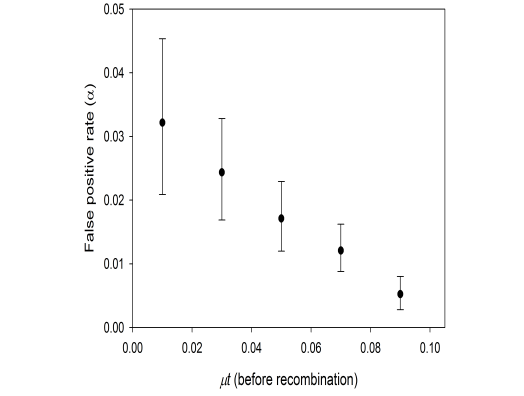
\includegraphics{Figures/HybridCheck/HC_FalseRate}
    \caption{\label{fig:HC_False}The mean($\pm$5 - 95\%CI) false positive rate ($\alpha$) of HybridCheck as a function of the ancestral divergence time $\mu t$ (i.e. the amount of time of the sequences diverged before recombination). As sequences become more diverged, the false positive rate decreases.}
\end{figure}

The false negative rate is presented in Figure~\ref{fig:HC_Power}. The false negative rate is plotted on the y-axis, against the amount of time since recombination occurred (expressed as $\mu t$). The data is partitioned into series, according to the amount of divergence (expressed as $\mu t$) between parental sequences prior to hybridisation. Figure n+1 shows that HybridCheck was able to detect $>$95\% of recent introgression events even if the two parental populations had diverged only moderately. However, more ancient introgression events were detected only if both parental populations had significantly diverged.

\begin{figure}
	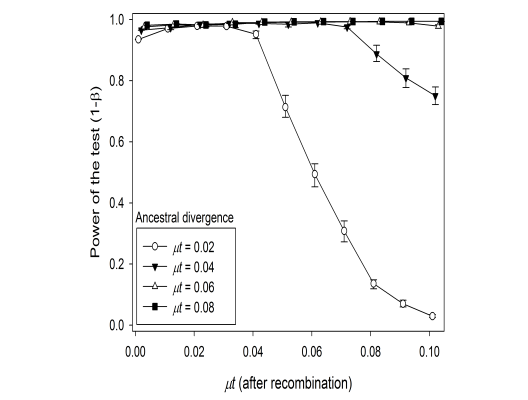
\includegraphics{Figures/HybridCheck/HC_Power}
    \caption{\label{fig:HC_Power}The mean($\pm$5 – 95\%CI) statistical power (1 - $\beta$) of HybridCheck as a function of the divergence time of the sequences after recombination (expressed in $\mu t$) for sequences with ancestral divergence times $\mu t$ = 0.2, 0.4, 0.6 and 0.8 generations. Recombination between moderately diverged sequences can be detected in $>$95\% of the cases, as long as the recombination event was relatively recent.}
\end{figure}

The accuracy of the dating estimates HybridCheck calculates for our simulated scenario is presented in Figure~\ref{fig:HC_Age}. This analysis shows that when the ancestral sequenced had diverged significantly ($\mu t \geq$ 0.2), the age estimates calculated by HybridCheck are a good approximation of the actual time passed since recombination (Linear Regression: Estimated age = 0.000795 + 0.968 t, R2=99.3\%). However, when the exchanges occurred between sequences that were only moderately diverged ($\mu t <$ 0.2), the age of the recombination events are underestimated when recombination happened in the distant past ($\mu t >$ 0.05) (see Figure~\ref{fig:HC_Age}). In such cases, mutations accumulated after the recombination event fragmented the blocks, resulting in an underestimate of the number of SNPs in the blocks that were detected.

\begin{figure}
	\includegraphics{Figures/HybridCheck/HC_Age}
    \caption{\label{fig:HC_Age}The mean ($\pm$SEM) estimated age (expressed in $\mu t$) of recombinant blocks calculated using the dating algorithm with a JC correction in HybridCheck, versus their actual age. In most of the scenarios, HybridCheck returns an unbiased estimate of the divergence time. However, the age is underestimated in cases of ancient recombination between populations that have ancestral divergence of 0.2.}
\end{figure}


\section{Discussion}
In this project, the objectives were to create and test a software package for the exploratory analysis of large sequences for evidence of introgression and hybridization. The package is designed to take the researcher through the following questions:

\begin{enumerate}
	\item Is there evidence of recombination / introgression?
    \item Where are the recombination regions in the sequences?
    \item What is the divergence time of recombinant blocks that are detected by the package?
\end{enumerate}

\subsection{Performance of detecting recombinant blocks}

The data demonstrate that for the simulated scenarios, HybridCheck performs best when sequences are diverged sufficiently prior to hybridization, and the hybridization or recombination event was relatively recent.
However, when the parental sequences of the hybrid sequence were sufficiently diverged recombinant blocks were clearly detected long after the recombination event ($\mu t >$ 0.06).
In addition, when divergence between parental sequences of a hybrid sequence was high then dating estimates of the recombinant blocks remained more accurate for older recombination blocks. 

If two parental sequences are significantly diverged prior to hybridisation, the introgressed regions will be more apparent in the sequence similarity scans of HybridCheck because their high nucleotide similarity stands in sharp contrast with the genomic background.
With a lower level of ancestral divergence, the increase in local sequence similarity caused by recombination is more difficult to distinguish from stochastic variation in nucleotide divergence, around a higher average level of sequence similarity.
As a result, the algorithm HybridCheck employs to decide on a suitable sequence similarity threshold can be confounded as it tries to identify regions with sequence similarity that fall outside of the mean noise levels of sequence similarity.
Therefore, HybridCheck would struggle to analyse a study system in which populations or taxa analysed are too closely related and have not diverged for long enough to accumulate unique polymorphisms which will be shared between parental and hybrid sequences. 

Previous studies have shown that many window based recombination detection methods perform better when the divergence is above ~0.05 (expressed as a proportion of the sequence length) \parencite{Posada2001b}.
Furthermore, simple implementations such as MAXCHI, and site incompatibility based methods usually perform better than phylogenetic based methods because the latter only tend to detect recombination if it changes the tree topology \parencite{Posada2001b}.

HybridCheck window scans attempt to find elevated similarity between genome sequences / contigs of two taxa which are unrelated.
Such elevations in similarity are indicative of, and often coincide with incongruence between differing gene tree topologies.
However, such signatures can have causes other than recombination, and elevated levels of sequence similarity could also be due to stabilizing selection conserving sequences between populations.
Alternatively, diverging populations of organisms could show increased levels of divergence in regions of the genome that are under adaptive selection, and if there is gene flow between populations the background will be homogenized compared to the regions that are subject to divergent selection \parencite{Nadeau2012}.
Such genomic islands of divergence appear to be less evident between populations that are further along the speciation process in butterfly species \parencite{Nadeau2012}.
A selective sweep is a phenomenon whereby positive selection in an allele reduces variation in neighboring regions due to linkage.
This is also called hitchhiking \parencite{Hedrick1980}.
If a selective sweep is strong and only one haplotype exists in high numbers in the population as a result, then a large reduction in variation is possible.
Selective sweeps could create regions of sequence similarity similar to those created by hybridisation events.
Note however, this scenario reduces variation around a positively selected allele within in a population.

HybridCheck attempts to overcomes these effects of selection in part by removing non-polymorphic sites prior to measuring the sequence similarity across sequences, but it is still possible that selection could be responsible, and the removal of informative sites by selection therefore reduces the power of HybridCheck to reliably identify introgression in those regions.
Therefore HybridCheck is not recommended or useful if a researcher is interested in smaller regions subject to very strong selection, due to the resulting lack of information.
If there are protein-coding regions in a detected recombinant region and selection is thought to be responsible, then the sequences should be analysed for evidence of purifying selection and/or selective sweeps within the detected region.

Elevated sequence similarity and incongruent tree topologies can also be caused by “incomplete lineage sorting” or deep coalescence \parencite{Rogers2014ComparativeDynamics}.
This occurs when an ancestral species is polymorphic for a given gene before the species tree splits into two daughter species.
After the first species split, if the polymorphism does not become resolved into two separate monophyletic lineages before the next speciation event, then the species tree will not match the gene trees of individual alleles \parencite{Rogers2014ComparativeDynamics}.
This problem is likely if a population size is very large, or if the time between branching events is low \parencite{Rogers2014ComparativeDynamics}.
Much of the genome of \textit{Homo sapiens} shows evidence of incomplete lineage sorting.
As a consequence, parts of the genome supported the phylogeny (chimpanzee, (human, gorilla)), whereas other regions of the genome supported the phylogeny (human, (chimpanzee, gorilla)) \parencite{Galtier2008}.
Both these phylogenies disagree with the species phylogeny of homonids (gorilla, (human, chimpanzee)) \parencite{Galtier2008,Rogers2014ComparativeDynamics}.
This discordance is because selection can cause similar sequences, or islands of divergence as previously described, and then incomplete lineage sorting results in gene trees that are discordant with the species tree and other gene trees, as a result of the incomplete and stochastic resolutions of polymorphisms, before subsequent speciation events \parencite{Scally2012}.

However, HybridCheck can help discern recombination from incomplete lineage sorting by comparing the coalescence time of recombinant regions with the split of the species.
If the age of a recombinant region is significantly younger than the split of the ancestral species, the pattern is inconsistent with incomplete lineage sorting.
In this case, genetic introgression after hybridisation is a more plausible explanation for the observed increase in local sequence similarity.
HybridCheck makes this practically possible for the researcher to do, for many recombinant blocks.

To summarise the performance of the HybridCheck when identifying recombinant regions, the HybridCheck use case is intended predominantly as an exploratory method to scan for signal between sequences from diverged populations or taxa, rather than within populations.
Outside of this use case, HybridCheck may be unsuitable for some systems as a result of limited divergence between sequences, and selection, both of which result in reduced information for the HybridCheck analysis method. 
Recent speciation and large population sizes may result in incomplete lineage sorting, which can affect patterns of divergence and ancestry in similar ways to recombination, however coalescent times computed by HybridCheck may help distinguish incomplete lineage sorting from recombination.
When using HybridCheck for a study system outside of its designed use case, whilst it is useful for highlighting the regions of the genome affected by the above factors, regions should not be uncritically considered the result of hybridisation or recombination, and the alternative causes e.g. selection should be followed up and ruled out before any such conclusion. 

\subsection{Performance of estimating the age of recombination events}
From the results it is evident that the dating algorithm used in HybridCheck tends to underestimate the divergence time of recombinant blocks in old recombination events. This is because recombination blocks can become fragmented by accumulation of subsequent mutations following the recombination event. Consequently, older recombination blocks tend to be smaller, when they are actually larger. Thus, not all mutations are accounted for, resulting in an underestimate of the divergence time particularly for old recombination events.

Furthermore, the dating algorithm used in HybridCheck makes several assumptions in order to be simple and fast. As a result however, if these assumptions are broken then this will affect how representative the estimates returned by HybridCheck are of the true age of a recombination event. The algorithm assumes that the mutation rate has been constant over time and identical in all taxa. This assumption is not always true, and more sophisticated approaches, such as the Fossilized-Birth-Death process allow for the calibration of divergence time estimates during Bayesian phylogeny estimation \parencite{Heath2014}. It uses all available fossils, and considers extant species and fossils of species part of the same macro-evolutionary process \parencite{Heath2014}.

In addition, the algorithm uses a nucleotide substitution rate to infer the mutation rate. In order to correct for mutation saturation, homoplasy, back mutations and transition / transversion ratios, HybridCheck converts the number of SNPs into the number of mutations using a JC \parencite{Jukes1969}, K80 \parencite{Kimura1980ASequences}, F81 \parencite{Felsenstein1981EvolutionaryApproach}, HKY \parencite{Hasegawa1985DatingDNA}, or GTR \parencite{Tavare1986SomeSequences} correction. However, substitution rates do not solely depend on mutation rates, and they appear to be auto-correlated across sequences due to the effect of selection. Selection can vary between sites, genes and taxa, and selection and substitution rates can change through time as conditions change \parencite{Barrick2013,Bromham2003a}.

Furthermore, the size of populations must be taken into account \parencite{Bromham2003a}. Bayesian coalescent approaches incorporated in software such as BEAST \parencite{Bouckaert2014BEASTAnalysis} should be used when using a relaxed clock or more advanced method of dating. However, these methods are computationally more demanding and might become unfeasible when estimating the divergence time of a large number of recombination events. In such cases, the age estimate returned by HybridCheck offers a good approximation when recombination occurred relatively recently ($\mu t <$ 0.05), and also when the ancestral sequences have diverged significantly before hybridizing.

In conclusion, the HybridCheck project is intended as a simple all-inclusive tool to analyse recombination in genome sequence data. The implemented algorithms are not as sophisticated as methods that employ Bayesian estimation of parameters and coalescent simulations. However, this means that the package is computationally fast, which makes it a useful first port-of-call for identifying recombination and assessing whether other explanations such as incomplete lineage sorting may apply.
